\documentclass{standalone}
\usepackage{tikz}
\usetikzlibrary{positioning,automata}

\begin{document}
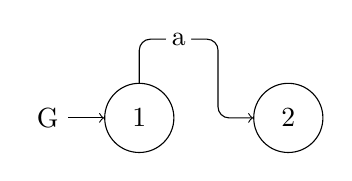
\begin{tikzpicture}
   \node[state,initial,initial text=G] (1)   {$1$}; 
   \node[state] (2) [right=of 1] {$2$}; 
   \draw[->,rounded corners] (1) |- node[pos=0.75,fill=white,inner sep=2pt]{a} ++(1,1) |- (2);
\end{tikzpicture}
\end{document}